\documentclass[12pt]{article}
\usepackage[margin=1in]{geometry}
\usepackage{graphicx}
\usepackage{blindtext}
\usepackage{mathtools}

\title{Graduate Student \LaTeX \ Tutorial}
\date{February 2016}
\author{Michael A. Herrera}

\begin{document}

\maketitle

\section{Introduction}

This tutorial was made for beginning users who don't have any experience in using \LaTeX.  This is not meant to be a comprehensive tutorial, but hopefully at the end, you will have enough information to continue learning on your own.  There are many different ways to accomplish similar tasks in \LaTeX \ and everything I know about \LaTeX is self taught, so the examples that I provide may not be optimal.  I have also made available the TeX file used to create this tutorial on my github account, https://github.com/mherr77m/LaTeX.

\section{Installation of \LaTeX}

There are two parts to a \LaTeX \ installation, the TeX distribution and the \LaTeX \ front end.  \LaTeX \ is a programming language, not a stand alone program.  The TeX distribution contains the source code for the language and a \LaTeX \ front end is where you will write and compile your code.  There are TeX distributions for all major operating systems and can be found at the following web address:

\begin{center}
https://latex-project.org/ftp.html
\end{center}

\noindent Once you have the distribution installed, you will need a front end where you can write your paper.  For this tutorial, I am using TeXShop which can be downloaded from here:

\begin{center}
http://pages.uoregon.edu/koch/texshop/obtaining.html
\end{center}

\noindent This editor is only available for Mac and is the same front end that is installed on the department computers.  If you would like a different editor, or if you are using another operating system, there are many other editors available, such as Texmaker:

\begin{center}
http://www.xm1math.net/texmaker/
\end{center}

\noindent The other option is to use an online \LaTeX \ editor.  These sites allow you to use \LaTeX \ without having to install it on your machine.  One example of these sites is Share LaTeX:

\begin{center}
https://www.sharelatex.com
\end{center}

\begin{figure}[b]
\centering
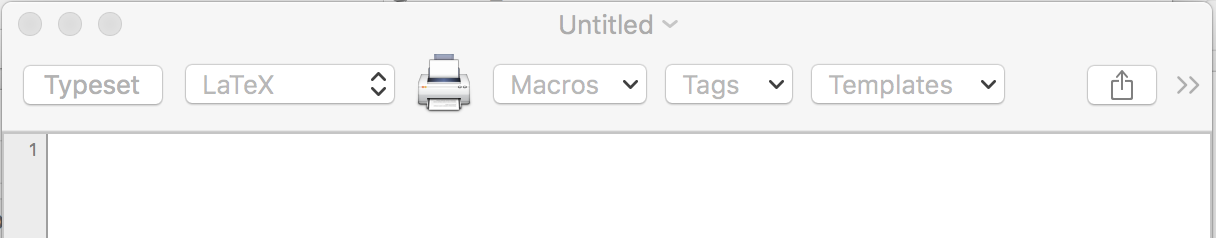
\includegraphics[width=0.9\textwidth]{env.png}
\caption{Example of the TeXShop environment.}
\label{env}
\end{figure}

\section{Staring a New Document}

When you open TeXShop, you are provided with a blank window in which to start writing your paper, Fig~\ref{env}.  \LaTeX \ is a compiled language, meaning that when you want to create a PDF of your paper, you will need to compile your code.  In TeXShop, to compile your code, you use the ``Typeset" button in Fig~\ref{env}.  There are different compiling options available in the pull down menu next to ``Typeset", but for now, we will leave it set to the default ``LaTeX" option.  If you aren't using any references in your text, you just need to compile the code twice, meaning that you use the ``Typeset" button twice.  This will link any equation and figure references you have in your text.

\subsection{Preamble}
The first thing that every \LaTeX \ document needs is a \textit{preamble}, which contains information that affects the entire document.  The general structure of a \LaTeX \ documents is,

\hfill

\noindent \verb!\documentclass{...}!\\
...\\
\verb!\begin{document}!\\
...\\
\verb!\end{document}!\\


\noindent Everything between the \verb!\documentclass{...}! and the \verb!\begin{document}! is called the \textit{preamble}.  This is where you will define your document type and load packages.  There are many different document types, such as article, book, and letter, but for most of us we will be using article class.  For this tutorial, your first command in your program should be 

\hfill

\noindent \verb!\documentclass[12pt]{article}!  

\hfill

\noindent Each command in \LaTeX \ is called by using a backslash \verb!\!.  Here, we have called the ``documentclass" command and passed it two arguments.  The argument in the curly brackets \verb!{ }! is the class type and any arguments in the square brackets \verb![ ]! are the class options.  There are multiple class options such as main font size, paper size, number of columns, etc.  An additional example of the document class command is seen below.

\hfill

\noindent \verb!\documentclass[10pt,a4paper,twocolumn]{article}!  

\hfill

\noindent Another part of the preamble is the loading of packages.  There are many packages included in the TeX distribution, but they are only loaded if you need them, very similar to importing in Python.  One of the most used packages is graphicx, which allows you to easily put figures into your paper.  If you want to change the margins of your paper, you can load the geometry package and set the margins.  You can load these packages by,

\hfill

\noindent \verb!\usepackage{graphicx}!  \\
\verb!\usepackage[margin=1in]{geometry}!

\hfill

\noindent where \verb!\usepackage{...}! is the command, ``geometry" is the argument passed to the command, and margin=1in is an argument specific to the geometry package.

\subsection{Title Page}

Now that we have defined our document and loaded a package,  we want to add a title page to our paper.  The first part of making a title is done in the preamble.  For the title page in this tutorial, the following three commands were used in the preamble.

\hfill

\noindent \verb!\title{Graduate Student \LaTeX \ Tutorial}!\\
\verb!\date{January 2015}!\\
\verb!\author{Michael A. Herrera}!

\hfill

\noindent Once you have defined the title, date, and author, you can call the \verb!\maketitle! command within the body of the code,

\hfill

\noindent\verb!\begin{document}!\\
\verb!\maketitle!\\
\verb!\newpage!\\
\verb!\end{document}!

\hfill

\noindent The \verb!\newpage! command will skip the rest of the page and start a new page.  Everything that we want to add from here on will be added to the body of the code, between \verb!\begin{document}! and  \verb!\end{document}!.

\section{Body of Text}

Once you have a title page, you can start the main body of your text.  One of the best ways to organize a paper is by sections as is seen in this tutorial.  The command to start a new section is \verb!\section{Section Title}!, where you replace ``Section Title" with the name of your section.  After you define a section, you can write the body of your paper just as you would in any other word processor.  If you want a section title without a number, you can add an asterisk to the command, \verb!\section*{Section Title}!.

\subsection{Sub-Section}

You also have the option of using sub-sections (\verb!\subsection{Sub-Section}!),

\subsubsection{Sub-Sub-Section}

and sub-sub-sections (\verb!\subsubsection{Sub-Sub-Section}!).

\subsection{Text Modifiers}

There are many different ways you can modify the text of your paper, such as \textbf{Bold}, \emph{italics}, or \LARGE font size. \normalsize I'm not going to go through every command you can use to alter text, but here is a list of some common commands:

\hfill
\large

\begin{tabular}{ l | c }
\textbf{Command} & \textbf{Result} \\ \hline
\verb!\textit{Italics}! & \textit{Italics} \\ \hline
\verb!\textbf{Bold}! & \textbf{Bold} \\ \hline
\verb!\texttt{Teletype Font}! & \texttt{Teletype Font} \\ \hline
\verb!\textsc{Small Capitals}! & \textsc{Small Capitals} \\ \hline
\verb!\uppercase{Uppercase}! & \uppercase{Uppercase} \\ \hline
\verb!\underline{Underline}! & \underline{Underline} \\ \hline
\verb!\tiny Tiny ! & \tiny Tiny  \\ \hline
\verb!\small Small ! & \small Small \\ \hline
\verb!\normalsize Normal Size ! & \normalsize Normal Size \\ \hline
\verb!\Large Large! & \Large Large \\ \hline
\verb!\Huge Huge! & \Huge Huge \\ \hline
\end{tabular}

\normalsize
\hfill \\

\noindent One thing to note about the font size commands is that you don't pass them any arguments.  Instead, you call the command and then all of the text afterwards will be at the new font size.  Once you want to return to the default font size, you can use the command \verb!\normalsize!.

The last thing I wanted to show in this section is creating lists, such as bullet points and numbered lists.  A simple bullet point list can be created using the following code,

\hfill

\noindent \verb!\begin{itemize}!\\
\verb!\item First bullet point!\\
\verb!\item Second bullet point!\\
\verb!\end{itemize}!

\hfill

\noindent which leads to,

\begin{itemize}
  \item First bullet point
  \item Second bullet point
\end{itemize}

\noindent If you want a numbered list you can use ``enumerate" instead of ``itemize",

\hfill

\noindent \verb!\begin{enumerate}!\\
\verb!\item First bullet point!\\
\verb!\item Second bullet point!\\
\verb!\end{enumerate}!

\hfill

\noindent which leads to,

\begin{enumerate}
  \item First bullet point
  \item Second bullet point
\end{enumerate}

\hfill

\noindent Finally, you can nest and combine these two types of lists,

\hfill

\noindent \verb!\begin{enumerate}!\\
\verb!\item First bullet point!\\
\verb!\item Second bullet point!\\
\verb!\begin{enumerate}!\\
\verb!\item Sub bullet point!\\ 
\verb!\begin{itemize}!\\
\verb!\item Sub sub bullet point!\\
\verb!\item Sub sub bullet point!\\
\verb!\end{itemize}!\\
\verb!\item Sub bullet point!\\
\verb!\end{enumerate}!\\
\verb!\end{enumerate}!

\hfill

\noindent which leads to,

\begin{enumerate}
\item First bullet point
\item Second bullet point
\begin{enumerate}
\item Sub bullet point 
\begin{itemize}
\item Sub sub bullet point
\item Sub sub bullet point
\end{itemize}
\item Sub bullet point
\end{enumerate}
\end{enumerate}

\hfill

\section{Equations}

Writing equations in \LaTeX \ is very different than other word processors.  Instead of using an equation editor to create an equation and then insert it into the paper, in \LaTeX \ you write your equations using \LaTeX \ commands.  To load all of the needed symbols and expressions, you can load the mathtools package in the preamble of the TeX file, \verb!\usepackage{mathtools}!.  

\subsection{In-Text Equations}

Sometimes equations are simple enough that you want to place them in the text, $p=\rho RT$, or you can use this same technique to explain terms in an equation, $\rho$ is density and $p$ is pressure.  To add an equation or use any math text within your text, you just need to surround the math expression in \verb!$...$!.  For example, the ideal gas law used earlier in this paragraph was created using \verb!$p=\rho RT$!.  

\subsection{Separate Equations}

The other way to write an equation is to place it on it's own line.  This is usually easier to read and allows for the equation to be referenced other places in the paper.  Using the ideal gas law from the previous example, we can rewrite the equation as,

\begin{equation}
p=\rho RT
\label{eq:one}
\end{equation}

\noindent You can see that the equation is now centered on it's own line and is numbered so that you can reference it in the paper.  The code used for the above equation was,

\hfill

\noindent \verb!\begin{equation}!\\
  \verb!p=\rho RT!\\
\verb!\label{eq:one}!\\
\verb!\end{equation}!

\hfill

\noindent The entire equation is wrapped in \verb!\begin{...}! and \verb!\end{...}! commands, with the actual equation in the middle.  The other part of this equation is the label, which allows you to reference the equation later in the paper, Eq~\ref{eq:one}, \verb!\ref{eq:one}!.

\subsection{Symbols}

There are a wide array of mathematical symbols and expressions available in \LaTeX \, allowing you to write just about any equation you want.  In this section, I've included some of the most commonly used expressions.  To use these examples, you just need to place the expressions between the begin and end commands, like in Eq~\ref{eq:one}.

The most basic math symbols that are available on you keyboard can be used normally in an equation, such as,

\hfill

$+\; -\; =\; !\; /\; (\; )\; [\; ]\; <\; >\; |\; '\; :$

\hfill

\noindent There are two ways to use parenthesis and square brackets.  If you you them normally, \verb!( )! or \verb![  ]!, you can get an equation that looks like this,

\begin{equation}
\theta = T(\frac{p_o}{p})^\kappa
\end{equation}

\noindent You can see that parenthesis are too small so to fix this issue, we can add the \verb!\left! and \verb!\right! commands before the parenthesis, \verb!\left ( ... \right )!, which results in the equation,

\begin{equation}
\theta = T\left(\frac{p_o}{p}\right)^\kappa.
\end{equation}

\hfill

\noindent Greek letters are also available and easy to use, \verb!\delta! becomes $\delta$ and \verb!\Delta! becomes $\Delta$.

\hfill

\begin{tabular}{l c | l c | l c | l c | l c}
\verb!\alpha! & $\alpha$ & \verb!\kappa! & $\kappa$ & \verb!\psi! & $\psi$ & \verb!\Delta! & $\Delta$ & \verb!\Theta! & $\Theta$\\
\verb!\beta! & $\beta$ & \verb!\lambda! & $\lambda$ & \verb!\rho! & $\rho$ & \verb!\Gamma! & $\Gamma$ &\verb!\Upsilon! & $\Upsilon$\\
\verb!\chi! & $\chi$ & \verb!\mu! & $\mu$ & \verb!\sigma! & $\sigma$ & \verb!\Lambda! & $\Lambda$ & \verb!\Xi! & $\Xi$\\
\verb!\delta! & $\delta$ & \verb!\nu! & $\nu$ & \verb!\tau! & $\tau$ & \verb!\Omega! & $\Omega$\\
\verb!\epsilon! & $\epsilon$ & \verb!o! & $o$ & \verb!\theta! & $\theta$ & \verb!\Phi! & $\Phi$\\
\verb!\eta! & $\eta$ & \verb!\omega! & $\omega$ & \verb!\upsilon! & $\upsilon$ & \verb!\Pi! & $\Pi$\\
\verb!\gamma! & $\gamma$ & \verb!\phi! & $\phi$ & \verb!\xi! & $\xi$ & \verb!\Psi! & $\Psi$\\
\verb!\iota! & $\iota$ & \verb!\pi! & $\pi$ & \verb!\zeta! & $\zeta$ & \verb!\Sigma! & $\Sigma$
\end{tabular}

\hfill

\noindent \\Fractions can be written using the \verb!\frac{numerator}{denominator}! command.

\hfill 

\noindent \verb!\begin{equation}!\\
\verb! q = \frac{r_v}{1+r_v}!\\
\verb!\end{equation}!

\hfill

\noindent Which produces,

\begin{equation}\\
q = \frac{r_v}{1+r_v}\\
\end{equation}\\

\noindent To add a subscript you can use an underscore followed by the subscript, \verb!_!.  If your subscript is more than a single character you can add curly brackets, \verb!_{...}!.  

\hfill

\begin{tabular}{l | c}
\verb!x_i! & $x_i$ \\
\verb!x_{i+1}! & $x_{i+1}$
\end{tabular}

\hfill

\noindent Superscripts are the same except the command is \verb!^! and if your superscript is multiple characters, \verb!^{...}!.  

\hfill

\begin{tabular}{l | c}
\verb!x^2! & $x^2$ \\
\verb!e^{x+1}! & $e^{x+1}$
\end{tabular}

\hfill

\noindent You can also combine subscripts and subscripts,

\hfill

\begin{tabular}{l | c}
\verb!x_i^2! & $x_i^2$ \\[5pt]
\verb!e_{i+1}^{x+1}! & $e_{i+1}^{x+1}$\\[5pt]
\verb!e_{i+1}^{x^2}! & $e_{i+1}^{x^2}$
\end{tabular}

\hfill

\noindent Square roots and nth roots are created using the \verb!\sqrt{...}! command,

\hfill

\begin{tabular}{l | c}
\verb!\sqrt{x+y}! & $\sqrt{x+y}$ \\[5pt]
\verb!\sqrt[3]{x+y}! & $\sqrt[3]{x+y}$
\end{tabular}

\noindent \\Sums are made using \verb!\sum{...}! and products are made using \verb!\prod{...}!.

\hfill

\noindent \verb!\sum_{n=1}^{N} n^2! produces,

\begin{equation}
\sum_{n=1}^{N} n^2
\end{equation}

\noindent and \verb!\prod_{n=1}^{N} n^2! produces,

\begin{equation}
\prod_{n=1}^{N} n^2 
\end{equation}

\noindent Integrals are very similar to sums and products, \verb!\int_{a}^{b} x^2 dx! results in,

\begin{equation}
\int_{a}^{b} x^2 dx
\end{equation}

\noindent If you want to place the limits of integration on top of the integral instead of next to it, you can use \verb!\int \limits_{a}^{b} x^2 dx!,

\begin{equation}
\int\limits_{a}^{b} x^2 dx
\end{equation}

\noindent Limits can be written by using \verb!\lim_{...}! command.  \verb!\lim_{x\to\infty} f(x)! produces,

\begin{equation}
\lim_{x\to\infty} f(x)
\end{equation}

\noindent One of the things you might have noticed is that characters used in an equation are a different font than normal text.  This means that if your equation has a cosine in it, if you where to just type out \verb!cos(\theta)!, your cosine would look like $cos(\theta)$.  However, we want our cosine to use the standard font, so we use the cosine command \verb!\cos!.

\hfill

\begin{tabular}{l c | l c}
\verb!\sin(\theta)! & $\sin(\theta)$ & \verb!\arcsin(\theta)! & $\arcsin(\theta)$ \\
\verb!\cos(\theta)! & $\cos(\theta)$ & \verb!\arccos(\theta)! & $\arccos(\theta)$ \\
\verb!\tan(\theta)! & $\tan(\theta)$ & \verb!\arctan(\theta)! & $\arctan(\theta)$ \\
\end{tabular}

\hfill

\section{Figures}

To include figures in your paper, you need the graphicx package, \verb!\usepackage{graphicx}!.  Inserting a figure is similar to inserting an equation, where you have a begin and end command.  Instead of passing ``equation" as an argument, you pass ``figure".

\hfill

\noindent \verb!\begin{figure}!\\
...\\
\verb!\end{figure}!

\hfill

Any commands pertaining to the figure goes in between the begin and end commands.  To add a figure, you use the \verb!\includegraphics[options]{figurename}! command, and pass the filename to the command.  If you don't include a file path to your figure, then the image must be in the same location as your .tex file.  One of the options you can pass is the desired size of the figure.  There are width and height options, if only one of them is set, then the aspect ratio of the figure is maintained.  Here is the code  used in inserting Figure~\ref{env} earlier in the tutorial.

\hfill

\noindent \verb!\begin{figure}[b]!\\
\verb!\centering!\\
\verb!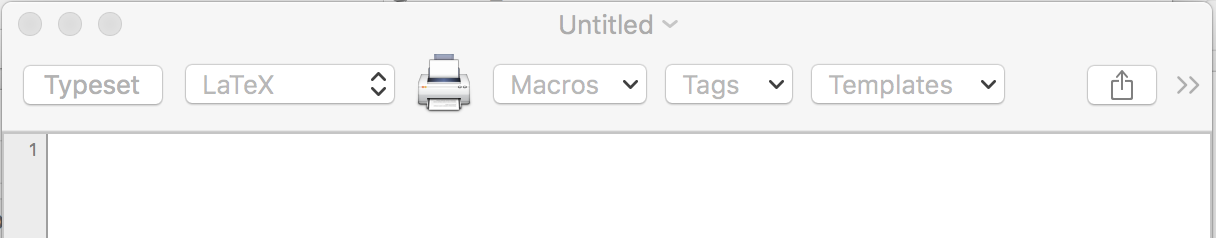
\includegraphics[width=0.9\textwidth]{env.png}!\\
\verb!\caption{Example of the TeXShop environment.}!\\
\verb!\label{env}!\\
\verb!\end{figure}!

\hfill

\noindent In the above example, the width of the figure is set to \verb![width=0.9\textwidth]!, which means that the figure will be rescaled so that it will take up 90\% of the width of the paper, excluding the margins.  If you don't set an width or height of the figure, the image will be inserted as the actual size of the image.  The \verb!\centering! command centers the figure in the paper, and the \verb![b]! option in the begin command tells \LaTeX \ to place the figure at the bottom of the page.  A note about the placement of figures, \LaTeX \ places the figure automatically on the page it feels works best.  Adding a caption to the figure is as easy as \verb!\caption{...}! and labeling works the same as with equations.

\section{Tables}

Inserting tables is just like inserting figures, but we now pass the argument ``tabular",

\hfill

\noindent \verb!\begin{tabular}{c c | c c}!\\
...\\
\verb!\end{tabular}!

\hfill

\noindent The other option that is passed in the above example is the number of columns in the table.  In this case there are four columns, center justified and a line between the second and third columns.  Each ``c" represents a center justified column and the pipe, ``$|$" adds a line between columns.  You can also make a column left justified by using an ``l" or right justified using an ``r" instead of ``c", but be careful not to confuse the pipe symbol ``$|$" and the letter ``l".  An example table can be made using,

\hfill

\noindent \verb!\begin{tabular}{c r | l c}!\\
\verb!1 & 2 & 3 & 4 \\!\\
\verb!a & b & c & d \\!\\
\verb!\hline!\\
\verb!$x$ & $y^2$ & $\rho$ & $\cos(\theta)$!\\
\verb!\end{tabular}!

\hfill

\noindent which produces,

\hfill

\begin{tabular}{c r | l c}
1 & 2 & 3 & 4 \\
a & b & c & d \\
\hline
$x$ & $y^2$ & $\rho$ & $\cos(\theta)$
\end{tabular}

\hfill

\noindent \\Each line after the begin command creates a new row in the table.  Each element of the row is separated by an \&.  After the last element, to create a new row you us a double backslash \verb!\\!.  If you want a horizontal line, you use the \verb!\hline! command.  Finally, the table can contain whatever you like, such as text, numbers, and equations, and the width of the columns will automatically adjust to fit.  

\section{Templates}

\LaTeX has the ability to use templates so you don't have to set up all the formatting yourself.  This section will focus on two templates, the American Meteorological Society template and the TAMU Thesis Office template, as well as how to use references in your paper.

\subsection{AMS Template}

For submissions to any of the AMS journals, like Monthly Weather Review (MWR) or the Journal of Atmospheric Sciences (JAS), you have to use the AMS template.  It can be downloaded from their website at,

\begin{center}
https://www2.ametsoc.org/ams/index.cfm/publications/authors/journal-and-bams-authors/author-resources/latex-author-info/
\end{center}

\noindent or from my github repository at https://github.com/mherr77m/LaTeX.

The directory that you download contains a bunch of files, but the important ones that you need for your paper are ametsoc.cls, ametsoc2014.bst, template.tex, and references.bib.  The template.tex file is where you will write your paper and references.bib is where you put your references.  The other two files are used for formatting and you shouldn't need to edit them.  

Let's start with the template.tex file which you can open using TexShop or your desired \LaTeX \ front end.  The first thing that you'll notice is all of the comments.  You can leave comments in your code by using \verb!%!.  The first actual command is defining the document class, which is now defined as ametsoc.  This is where you tell \LaTeX \ that you want to use the AMS template.  The next command \verb!\journal{...}! lets you define which journal you are submitted to, since they don't all use the exact same formatting.  Lines 53 through 91 help you set up your title page.  The last part of the preamble is the abstract and all you have to do is put the text of your abstract within the \verb!\abstract{...}! command.

The main body of the paper is where you will write your paper using all of the tools discussed earlier in this tutorial.  The template also has areas for acknowledgments and appendixes.  AMS journals request that you put all the tables and figure at the end of the paper, so from line 186 to the end is where you would place your tables and figures.

\subsubsection{References}

A very important thing you need to do to make sure your references work in the template is to uncomment lines 182 and 183, \verb!\bibliographystyle{ametsoc2014}! and \\\verb!\bibliography{references}!.  These two lines establish the formatting for the bibliography and the finds your references.  In the template directory, you references will be put into references.bib.

When you open references.bib in TexShop, the top half of the file contains a long list of journal name abbreviations that you can use when defining your references.  At the bottom are sample references that you can delete and replace with your own references.  For this tutorial, I'm only going to discuss one type of reference, a journal article.  Here is an example reference definition,

\hfill

\verb!@article{Lorenz1969,! \\
\verb!         author = {E. N. Lorenz},! \\
\verb!         title = {Predictability of a flow which possesses many scales of motion},! \\
\verb!         journal = TELLUS,!\\
\verb!         year = {1969},!\\
\verb!         volume = 21,!\\
\verb!         pages = {289--307}}!\\

\hfill

The first line is the type of reference, in this case a journal article, which you pass several arguments describing the article.  The first argument, \verb!Lorenz1969b! is the label for the reference.  When you want to use this reference in the paper, you will use this label.  The next two lines are for the authors and title.  The journal argument is where you can use the abbreviations from above, in this case it's not really an abbreviation since the journal name is short.  The final three lines are self explanatory, they are for year, volume, and page numbers of the journal article.

You add all of your references like this to the bottom of references.bib.  The way that referencing works in \LaTeX \ is that when you compile your paper, the program looks through your references.bib file for the label and then puts the reference into your paper.  This means that your references don't have to be in any specific order and you can even have references that you don't end up using in the paper.  

Using the AMS template, there are two commands you can use in your paper to add citations, either \verb!\citet[...]{...}! or \verb!\citep[...]{...}!.  Here are some sample citation commands and how they will appear in the paper,

\hfill

\begin{tabular}{l | l}
\verb!\citet{jon90}! & Jones et al. (1990)\\
\verb!\citet[chap. 2]{jon90}! & Jones et al. (1990, chap. 2)\\
\verb!\citep{jon90}! & (Jones et al. 1990)\\
\verb!\citep[chap. 2]{jon90}! & (Jones et al. 1990, chap. 2)\\
\verb!\citep[see][]{jon90}! & (see Jones et al. 1990)\\
\verb!\citep[see][chap. 2]{jon90}! & (see Jones et al. 1990, chap. 2)\\
\hline
\verb!\citet{jon90,jam91}! & Jones et al. (1990); James et al. (1991) \\ 
\verb!\citep{jon90,jam91}! & (Jones et al. 1990; James et al. 1991) \\ 
\verb!\citep{jon90,jon91}! & (Jones et al. 1990,1991) 
\end{tabular}

\hfill

\noindent The final part of using citations is how to compile \LaTeX \ with references.  If you are using TexShop, you'll first have to ``Typeset" using LaTeX from the drop down menu seen in Figure~\ref{env}.  Once that is finished compiling, you'll change the LaTeX option to ``BibTex" and then typeset/compile again.  This compilation should be very quick, then you'll chose LaTeX from the drop down menu once again and compile two more times.  These are all the basics for using the AMS template.  

\subsection{Thesis Template}

The TAMU thesis template is a bit different from the AMS template, and can be found either in my github repository, or from 

\begin{center}
http://howdy.me
\end{center}

A large difference with this template is that it is much more modular than the AMS template.  You'll notice that there are several .tex files, luckily they are all named so that you know what each file is used for.  The main .tex file is tamuthesis.tex, which is the file you will compile.  You will not have to modify this file very often.  The first changes that need to be made start on line 55 and goes through line 68.  This is where you define your title, author, committee, etc.  After you define your title page, there are several \verb!\include! commands which are used to call the other .tex files.  For example, you will write your abstract in abstract.tex, then tamuthesis.tex will compile the abstract and add it to the main paper.  The only other thing you should need to change is to include additional sections as you need them, since only three are included in this template.  

The other .tex files are where you will actually write your paper.  Each .tex file already has some example text in them, so it is fairly straight forward on how to edit them and add your text.  One thing to notice is that figures are now placed in a ``figures" directory, so you'll need to make sure to include the directory name when inserting the figures.  For an example of this, see line 34 of section1.tex.  

References in this template are similar to the AMS template.  There is a references.bib file which contains lots of sample references.  You can add your references to this file and then cite them in your paper just like you would for the AMS template.  When you are ready to compile, you will compile tamuthesis.tex and you will compile it the same was as for an AMS paper.

\section{Wrap Up}

This tutorial only covered the basics of how to use \LaTeX \ to write your journal article or thesis.  There are many resources for any other questions you have.  If you have a problem in \LaTeX \ there is a good chance someone else has had the same problem and has solved it.  Here are some websites to check out for more help.

\begin{center}
https://en.wikibooks.org/wiki/LaTeX\\
https://www.sharelatex.com/learn/Main\_Page \\
http://tex.stackexchange.com/help\\
https://latex-project.org/ftp.html 
\end{center}

\end{document}



















